\documentclass{scalatekids-article}
\begin{document}
\lfoot{Analisi dei Requisiti 0.0.1}
\newgeometry{top=3.5cm}
\begin{titlepage}
  \begin{center}
    \begin{center}
      
\includegraphics[width=10cm]{sklogo.png}
    \end{center}
    \vspace{1cm}
    \begin{Huge}
      \begin{center}
        \textbf{Analisi dei Requisiti}
      \end{center}
    \end{Huge}
    \vspace{11pt}
    \bgroup
    \def\arraystretch{1.3}
    \begin{tabular}{r|l}
      \multicolumn{2}{c}{\textbf{Informazioni sul documento}} \\
      \hline
      \setbox0=\hbox{0.0.1\unskip}\ifdim\wd0=0pt
      \\
      \else
      \textbf{Versione} & 0.0.3\\
      \fi
      \textbf{Redazione} & \multiLineCell[t]{Redattore}\\
      \textbf{Verifica} & \multiLineCell[t]{Verificatore}\\
      \textbf{Approvazione} & \multiLineCell[t]{Approvatore}\\
      \textbf{Uso} & Esterno\\
      \textbf{Lista di Distribuzione} & \multiLineCell[t]{ScalateKids\\Prof. Tullio Vardanega\\Prof. Riccardo Cardin}\\
    \end{tabular}
    \egroup
    \vspace{22pt}
  \end{center}
\end{titlepage}
\restoregeometry
\clearpage
\setcounter{page}{1}
\begin{flushleft}
  \vspace{0cm}
         {\large\bfseries Diario delle modifiche \par}
\end{flushleft}
\vspace{0cm}
\begin{center}
  \begin{tabular}{| l | l | l | l | l |}
    \hline
    Versione & Autore & Ruolo & Data & Descrizione \\
    \hline
    0.0.1 & Andrea Giacomo Baldan & & 2015-12-27 & Creazione scheletro del documento\\
    \hline
  \end{tabular}
\end{center}
\tableofcontents
\newpage
\section{Sommario}
\subsection{Scopo del documento}
Il seguente documento ha lo scopo di presentare le funzionalità che il prodotto
\textbf{Actorbase} esporrà all'utilizzatore finale. Inoltre elenca e descrive i
requisiti derivanti dalle suddette funzionalità, emersi durante le riunioni
interne ed esterne con il proponente.
\prodPurpose \glossExpl
\subsection{Riferimenti}
\subsubsection{Normativi}
\begin{itemize}
\item\textbf{Capitolato d'appalto C1:} \textit{Actorbase: a NoSQL DB based on the Actor model}\\
  \url{http://www.math.unipd.it/~tullio/IS-1/2015/Progetto/C1.pdf}
\item\textbf{Verbale esterno:} % TODO link
\item\textbf{Norme di Progetto:} % TODO link
\end{itemize}
\subsubsection{Informativi}
\begin{itemize}
\item\textbf{Dispense fornite dall'insegnamento Ingegneria del Software mod. A:}\\
  \url{http://www.math.unipd.it/~tullio/IS-1/2015/Dispense/L06.pdf}
\item\textbf{Dispense fornite dall'insegnamento Ingegneria del Software mod. A:}\\
  \url{http://www.math.unipd.it/~tullio/IS-1/2015/Dispense/E02.pdf}
\item\textbf{CAP theorem:}\\ % TODO: da inserire?
  \url{https://en.wikipedia.org/wiki/CAP_theorem}
\item\textbf{Reactive Manifesto:}
  \url{http://www.reactivemanifesto.org/}
  \url{https://en.wikipedia.org/wiki/Reactive_programming}
\item\textbf{Amazon DynamoDB:}
  \url{http://docs.aws.amazon.com/amazondynamodb/latest/developerguide/Introduction.html}
\end{itemize}
\section{Descrizione generale}
\subsection{Prospettive del prodotto}
l'obiettivo del prodotto è fornire un database \gloss{NoSQL} di tipo
\gloss{key-value}, quindi senza schemi predefiniti e tabelle; che utilizzi il
modello ad attori per garantire un alto grado di \gloss{concorrenza} e
\gloss{scalabilità orizzontale} idealmente illimitata.
\subsection{Funzioni}
Il software fornirà un sistema di interazione con l'utente basata su \gloss{ui}
testuale direttamente da riga di comando. Permetterà di effettuare le operazioni
basilari che ogni database fornisce:
\begin{itemize}
\item Creazione di una o più collezioni;
\item Cancellazione di una o più collezioni;
\item Modifica di una collezione;
\item Ricerca all'interno del database o all'interno di una o più collezioni;
\item Inserimento;
\item Cancellazione;
\item Aggiornamento;
\item Importazione ed esportazione di dati in formato \gloss{JSON}. % TODO: controllare
\end{itemize}
Il programma inoltre permetterà la richiesta di un aiuto esplicativo sull'uso
dei comandi.
\subsection{Caratteristiche utenza}
Il prodotto è orientato all'utilizzo da parte di clientela interessata a
sviluppo di applicazioni \gloss{reactive}, che trattino grandi moli di dati e
debbano fornire brevissimi tempi di risposta, sacrificando dunque le
funzionalità relazionali tipiche dei tradizionali database \textit{SQL} in
favore di un sistema fortemente \gloss{concorrente} e senza l'\gloss{overhead} generato
dagli schemi \gloss{SQL}.
\subsection{Vincoli}
Per far funzionare \textbf{Actorbase} è necessario disporre di un computer con
installata la \textit{\gloss{JVM} versione 8}. Non ci sono ulteriori richieste h
ardware o software.
\section{Casi d'uso}
Le aspettative di esperienza utente derivano dall'utilizzo da parte dei
componenti del gruppo di \gloss{Amazon DynamoDB}, un database \gloss{key-value}
sviluppato da \textit{Amazon}, utilizzato come modello di riferimento per lo
sviluppo. I casi d'uso seguono le norme di stesura elencate nel documento \textit{Norme di Progetto}.% TODO
                                                                                                     % link
\subsection{UC1: Interazioni basilari}
\begin{figure}[H]
  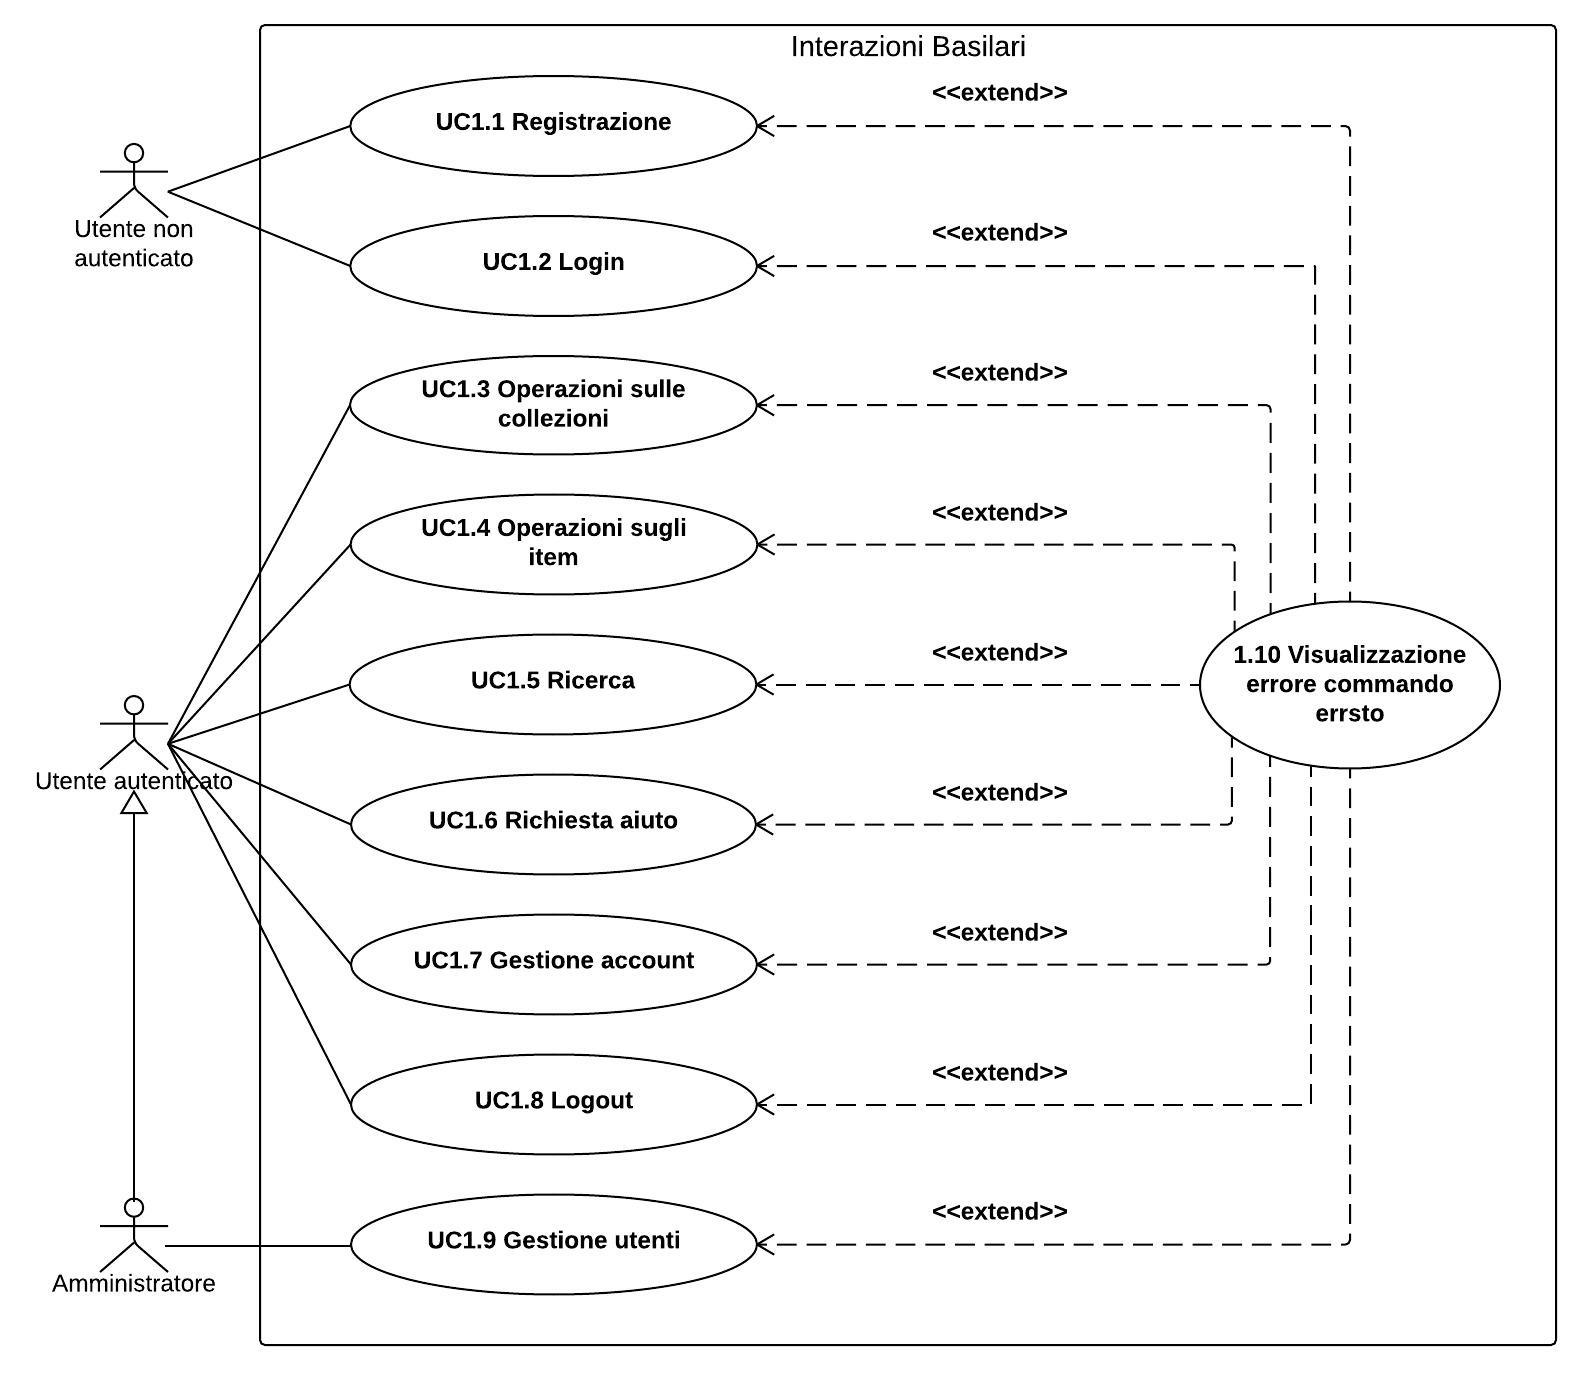
\includegraphics[width=0.7\textwidth,keepaspectratio]{UseCases/InterazioniBasilari.jpeg}
  \caption{Caso d'uso 1: Interazioni basilari}
\end{figure}
\textbf{Attori primari:} Utente\\ \\
\textbf{Scopo e descrizione:} Il database è installato correttamente e il server è in ascolto.
L'utente ha avviato un terminale ed è pronto ad inserire comandi.\\ \\
\textbf{Precondizione:} Il database è installato correttamente, e il server è in ascolto.\\ \\
\textbf{Flusso eventi:}
\begin{itemize}
\item UC1.1 Utente digita comando
\item UC1.2 Utente conferma il comando
\end{itemize}
\textbf{Postcondizione:} Il sistema ha prodotto l'output corrispondente al comando immesso dall'utente.
\subsection{UC1.1: Scrittura comando}

\textbf{Attori primari:} Utente\\ \\
\textbf{Scopo e descrizione:} L’utente scrive il comando sul terminale.\\ \\
\textbf{Precondizione:} Il database è installato correttamente, il server è in ascolto e l'utente intende scrivere un comando.\\ \\
\textbf{Flusso eventi:}
\begin{itemize}
\item UC1.1.1 Creazione di una collezione
\item UC1.1.2 Elencazione di collezioni
\item UC1.1.3 Cancellazione di una o più collezioni
\item UC1.1.4 Modifica di una collezione
\item UC1.1.5 Ricerca generale
\item UC1.1.6 Inserimento di un item
\item UC1.1.7 Cancellazione di un item
\item UC1.1.8 Modifica di un item
\item UC1.1.9 Richiesta di supporto
\end{itemize}
\textbf{Estensioni:}
\begin{itemize}
\item Nel caso in cui l'utente utilizzi un comando sconosciuto:
  \begin{itemize}
  \item viene visualizzato un messaggio di errore esplicativo (e rimando all'aiuto)
  \end{itemize}
\item Nel caso in cui l'utente utilizzi un comando conosciuto ma con parametri errati:
  \begin{itemize}
  \item viene visualizzato un messaggio di supporto che indica come usare correttamente il comando
  \end{itemize}
\item Nel caso in cui l'utente voglia modificare dati non presenti nel database:
  \begin{itemize}
  \item viene visualizzato un messaggio di errore esplicativo
  \end{itemize}
\end{itemize}
\textbf{Postcondizione:} L'utente ha digitato un comando
\subsection{UC1.1.1: Creazione di una collezione}
\textbf{Attore primario:} Utente\\ \\
\textbf{Scopo e descrizione:} L’utente intende creare una nuova collezione, deve inserire il nome della collezione.\\ \\
\textbf{Precodizione:} Il database è pronto a ricevere comandi e l’utente vuole creare una nuova collezione\\ \\
\textbf{Flusso di eventi:}
\begin{itemize}
\item l'utente digita il comando di creazione con parametro nome della nuova collezione
\end{itemize}
\textbf{Postcondizione:} L'utente ha digitato il comando per creare una collezione
\subsection{UC1.1.2: Elencazione di collezioni}
\textbf{Attore primario:} Utente\\ \\
\textbf{Scopo e descrizione:} L’utente intende elencare tutte le collezioni presenti nel database.\\ \\
\textbf{Precodizione:} Il database è pronto a ricevere comandi e l’utente vuole visualizzare un elenco delle collezioni\\ \\
\textbf{Flusso di eventi:}
\begin{itemize}
\item l'utente digita il comando di elencazione di collezioni
\end{itemize}
\textbf{Postcondizione:} L'utente ha digitato il comando per elencare le collezioni
\subsection{UC1.1.3: Cancellazione di una o più collezioni}
\textbf{Attore primario:} Utente\\ \\
\textbf{Scopo e descrizione:} L’utente intende cancellare una o più collezioni presenti nel database.\\ \\
\textbf{Precodizione:} Il database è pronto a ricevere comandi e l’utente intende cancellare una o più collezioni\\ \\
\textbf{Flusso di eventi:}
\begin{itemize}
\item l'utente digita il comando di cancellazione di una o più collezioni
\end{itemize}
\textbf{Postcondizione:} L’utente ha digitato il comando per cancellare una o più collezioni
\subsection{UC1.1.4: Modifica di una collezione}
\textbf{Attore primario:} Utente \\ \\
\textbf{Scopo e descrizione:} L’utente intende modificare una collezione, deve inserire i parametri per la modifica della collezione\\ \\
\textbf{Precondizione:} Il database è pronto a ricevere comandi e l’utente vuole modificare una collezione\\ \\
\textbf{Flusso di eventi:}
\begin{itemize}
\item l’utente digita il comando di modifica con parametri nome della collezione da modificare e valori dei campi da modificare
\end{itemize}
\textbf{Postcondizione:} L’utente ha digitato il comando per modificare una collezione
\subsection{UC1.1.5: Ricerca generale}

\textbf{Attore primario:} Utente \\ \\
\textbf{Scopo e descrizione:} L’utente intende effettuare una ricerca\\ \\
\textbf{Precondizione:} Il database è pronto a ricevere comandi e l’utente intende effettuare una ricerca\\ \\
\textbf{Flusso di eventi:}
\begin{itemize}
\item UC1.1.5.1 Utente può digitare il comando per effettuare una ricerca sull’intera base di dati
\item UC1.1.5.2 Utente può digitare il comando per effettuare una ricerca all’interno di una o più collezioni specifiche
\end{itemize}
\textbf{Postcondizione:} L’utente ha digitato il comando per effettuare una ricerca
\subsection{UC1.1.5.1: Ricerca all'interno della base di dati}
\textbf{Attore primario:} Utente \\ \\
\textbf{Scopo e descrizione:} L’utente intende effettuare una ricerca sull’intera base di dati\\ \\
\textbf{Precondizione:} Il database è pronto a ricevere comandi e l’utente intende effettuare una ricerca generale\\ \\
\textbf{Flusso di eventi:}
\begin{itemize}
\item l’utente digita il comando di ricerca generale
\end{itemize}
\textbf{Postcondizione:} L’utente ha digitato il comando per effettuare una ricerca di aiutanza generale
\subsection{UC1.1.5.2: Ricerca all'interno di una specifica collezione(o più)}
\textbf{Attore primario:} Utente \\ \\
\textbf{Scopo e descrizione:} L’utente intende effettuare una ricerca all’interno di una o più collezioni specifiche\\ \\
\textbf{Precondizione:} Il database è pronto a ricevere comandi e l’utente intende effettuare una ricerca dettagliata\\ \\
\textbf{Flusso di eventi:}
\begin{itemize}
\item l’utente digita il comando di ricerca con parametro i nomi delle collezioni sulle quali vuole effettuare la ricerca
\end{itemize}
\textbf{Postcondizione:} L’utente ha digitato il comando per effettuare una ricerca specifica
\subsection{UC1.1.6: Inserimento di un item}
\textbf{Attore primario:} Utente \\ \\
\textbf{Scopo e descrizione:} L’utente intende inserire un nuovo item in una collezione, deve inserire il nome della collezione e il nome dell’item\\ \\
\textbf{Precondizione:} Il database è pronto a ricevere comandi e l’utente vuole inserire un nuovo item in una collezione\\ \\
\textbf{Flusso di eventi:}
\begin{itemize}
\item l’utente digita il comando di inserimento con parametro nome della collezione e nome dell’item e campi dell’item
\end{itemize}
\textbf{Postcondizione:} L’utente ha digitato il comando per inserire un item
\subsection{UC1.1.7: Cancellazione di un item}
\textbf{Attore primario:} Utente \\ \\
\textbf{Scopo e descrizione:} L’utente intende cancellare un item da una collezione, deve inserire il nome dell’item da cancellare e il nome della collezione\\ \\
\textbf{Precondizione:} Il database è pronto a ricevere comandi e l’utente vuole cancellare un item da una collezione\\ \\
\textbf{Flusso di eventi:}
\begin{itemize}
\item l’utente digita il comando di cancellazione con parametro nome dell’item e della collezione
\end{itemize}
\textbf{Postcondizione:} l’utente ha digitato il comando per cancellare un item da una collezione
\subsection{UC1.1.8: Modifica di un item}
\textbf{Attore primario:} Utente \\ \\
\textbf{Scopo e descrizione:} L’utente intende modificare un item di una collezione, deve inserire il nome dell’item e della collezione\\ \\
\textbf{Precondizione:} Il database è pronto a ricevere comandi e l’utente vuole modificare un item di una collezione\\ \\
\textbf{Flusso di eventi:}
\begin{itemize}
\item l’utente digita il comando di modifica con parametro nome dell’item e della collezione
\end{itemize}
\textbf{Postcondizione:} L’utente ha digitato il comando per modificare un item
\subsection{UC1.1.9: Richiesta di supporto}

\textbf{Attore primario:} Utente \\ \\
\textbf{Scopo e descrizione:} L’utente intende richiedere del supporto\\ \\
\textbf{Precondizione:} Il database è pronto a ricevere comandi e l’utente intende richiedere supporto\\ \\
\textbf{Flusso di eventi:}
\begin{itemize}
\item UC1.1.9.1 Utente può digitare il comando per richiedere un aiuto generale
\item UC1.1.9.2 Utente può digitare il comando per richiedere un aiuto riguardo un particolare comando
\end{itemize}
\textbf{Postcondizione:} L’utente ha digitato il comando per richiedere supporto
\subsection{UC1.1.9.1: Richiesta di aiuto generale}
\textbf{Attore primario:} Utente \\ \\
\textbf{Scopo e descrizione:} L’utente intende richiedere del supporto generale\\ \\
\textbf{Precondizione:} Il database è pronto a ricevere comandi e l’utente intende richiedere supporto generale\\ \\
\textbf{Flusso di eventi:}
\begin{itemize}
\item L’utente digita il comando di aiuto con parametro nullo
\end{itemize}
\textbf{Postcondizione:} L’utente ha digitato il comando per richiedere supporto generale
\subsection{UC1.1.9.2: Richiesta di aiuto specifico}
\textbf{Attore primario:} Utente \\ \\
\textbf{Scopo e descrizione:} L’utente intende richiedere dell’aiuto su di un specifico comando\\ \\
\textbf{Precondizione:} Il database è pronto a ricevere comandi e l’utente intende richiedere supporto specifico\\ \\
\textbf{Flusso di eventi:}
\begin{itemize}
\item L’utente digita il comando di aiuto con parametro il comando di cui si vuole ricevere del supporto
\end{itemize}
\textbf{Postcondizione:} L’utente ha digitato il comando per richiedere supporto specifico
\subsection{UC1.2: Richiesta di aiuto specifico}

\textbf{Attore primario:} Utente \\ \\
\textbf{Scopo e descrizione:}  L’utente ha digitato un comando nella CLI con l’intenzione di inserire, cancellare, aggiornare, ricercare collezioni o item, o semplicemente per richiedere auto\\ \\
\textbf{Precondizione:} L’utente ha digitato un comando\\ \\
\textbf{Flusso di eventi:}
\begin{itemize}
\item L’utente conferma il comando digitato
\item UC 1.2.1 Il sistema esegue il comando immesso dall’utente
\end{itemize}
\textbf{Estensioni:}
\begin{itemize}
\item Nel caso in cui l’utente abbia utilizzato un comando sconosciuto:
  \begin{itemize}
  \item Viene visualizzato un messaggio di errore esplicativo (e rimando all'aiuto)
  \end{itemize}
\item Nel caso in cui l’utente abbia utilizzato un comando conosciuto ma con parametri errati:
  \begin{itemize}
  \item viene visualizzato un messaggio di supporto che indica come usare correttamente il comando
  \end{itemize}
\item Nel caso in cui l’utente abbia voluto modificare dati non presenti nel database:
  \begin{itemize}
  \item viene visualizzato un messaggio di errore esplicativo
  \end{itemize}
\end{itemize}
\textbf{Postcondizione:} Il sistema ha eseguito l’operazione richiesta dall’utente
% TODO: rispettare codici norme
\end{document}
